\documentclass[border=10pt]{standalone}
\usepackage{pgfplots}
\pgfplotsset{compat=1.17}
\begin{document}
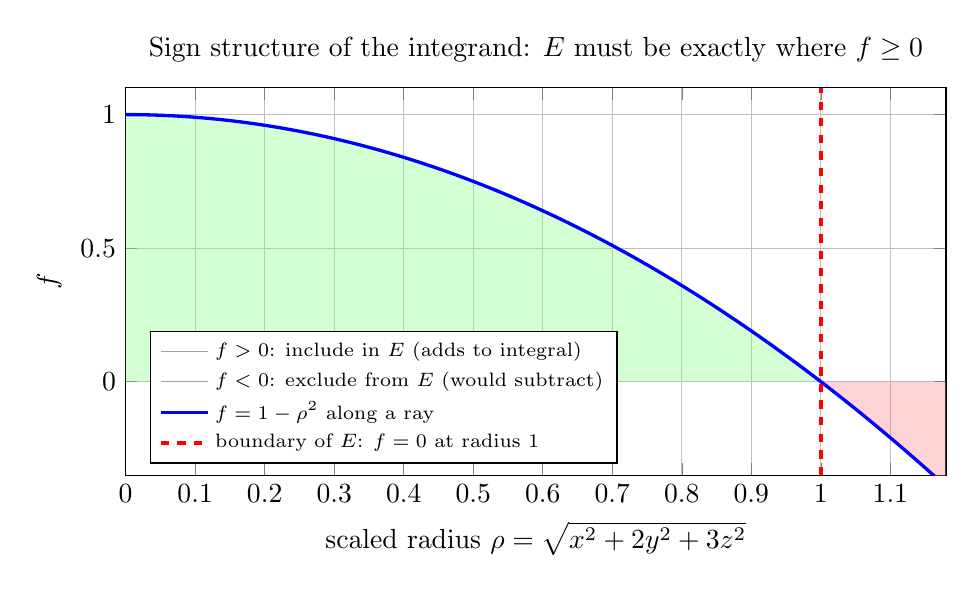
\begin{tikzpicture}
\begin{axis}[
    width=12cm, height=6.5cm,
    xlabel={scaled radius $\rho=\sqrt{x^2+2y^2+3z^2}$},
    ylabel={$f$},
    title={Sign structure of the integrand: $E$ must be exactly where $f\ge 0$},
    xmin=0, xmax=1.18, ymin=-0.35, ymax=1.1,
    grid=major,
    legend pos=south west,
    legend cell align=left,
    legend style={font=\scriptsize},
    samples=100,
]
% positive fill
\addplot[draw=none, fill=green!50, opacity=0.35, domain=0:1] {1-x^2} \closedcycle;
\addlegendentry{$f>0$: include in $E$ (adds to integral)}
% negative fill
\addplot[draw=none, fill=red!50, opacity=0.35, domain=1:1.18] {1-x^2} \closedcycle;
\addlegendentry{$f<0$: exclude from $E$ (would subtract)}
% curve
\addplot[blue, very thick, domain=0:1.18] {1-x^2};
\addlegendentry{$f = 1-\rho^2$ along a ray}
% boundary line
\addplot[red, dashed, very thick] coordinates {(1,-0.35) (1,1.1)};
\addlegendentry{boundary of $E$: $f=0$ at radius 1}
\end{axis}
\end{tikzpicture}
\end{document}